% Copyright (c) 2024 Alexander Bluhm <bluhm@genua.de>
%
% Permission to use, copy, modify, and distribute this software for any
% purpose with or without fee is hereby granted, provided that the above
% copyright notice and this permission notice appear in all copies.
%
% THE SOFTWARE IS PROVIDED "AS IS" AND THE AUTHOR DISCLAIMS ALL WARRANTIES
% WITH REGARD TO THIS SOFTWARE INCLUDING ALL IMPLIED WARRANTIES OF
% MERCHANTABILITY AND FITNESS. IN NO EVENT SHALL THE AUTHOR BE LIABLE FOR
% ANY SPECIAL, DIRECT, INDIRECT, OR CONSEQUENTIAL DAMAGES OR ANY DAMAGES
% WHATSOEVER RESULTING FROM LOSS OF USE, DATA OR PROFITS, WHETHER IN AN
% ACTION OF CONTRACT, NEGLIGENCE OR OTHER TORTIOUS ACTION, ARISING OUT OF
% OR IN CONNECTION WITH THE USE OR PERFORMANCE OF THIS SOFTWARE.

\documentclass[14pt]{beamer}
\usetheme{Frankfurt}
\usepackage{tikz}
\usepackage{framed}
\usepackage{graphicx}
\usepackage{varwidth}
\usepackage{tipa}
\usepackage{alltt}
\usepackage{xcolor}
\usepackage{upquote}
\usepackage[T1]{fontenc}
\usepackage{textcomp}
\usetikzlibrary{shapes.arrows}
\usetikzlibrary{shapes.geometric}
\usetikzlibrary{shapes.multipart}
\usetikzlibrary{shapes.symbols}
\author{Alexander Bluhm}
\title{A Packet's Journey Through the OpenBSD Network Stack}
\institute{genua GmbH\\ \url{bluhm@genua.de}\\ \url{bluhm@openbsd.org}}
\date{September 2024}
\let\Tiny\tiny

\begin{document}

\begin{frame}
\titlepage
\end{frame}

\setcounter{tocdepth}{1}
\section{Networking}
\begin{frame}{Agenda}
\tableofcontents[currentsection]
\end{frame}

\subsection{Environment}
\begin{frame}{Environment}
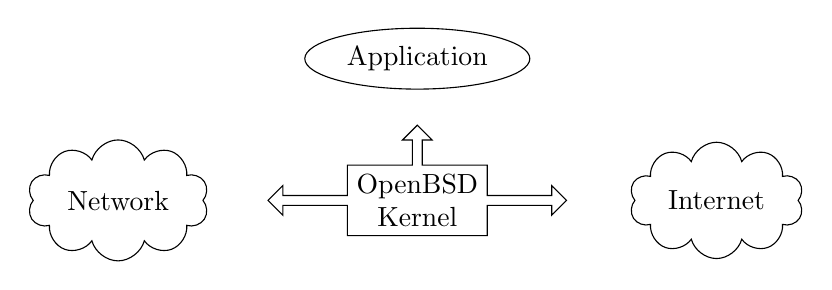
\begin{tikzpicture}
  \node [cloud, draw, aspect=2]
    at (-3.8, 0)
    {Network};
  \node [align=center, arrow box, draw,
    arrow box arrows={east:1cm, north:.5cm, west:1cm}]
    at (0, 0)
    {\begin{varwidth}{\textwidth}\centering OpenBSD \\ Kernel\end{varwidth}};
  \node [cloud, draw, aspect=2]
    at (3.8, 0)
    {Internet};
  \node [ellipse, draw, aspect=2]
    at (0, 1.8)
    {Application};
\end{tikzpicture}
\end{frame}

\subsection{Layer}
\begin{frame}{Layer}
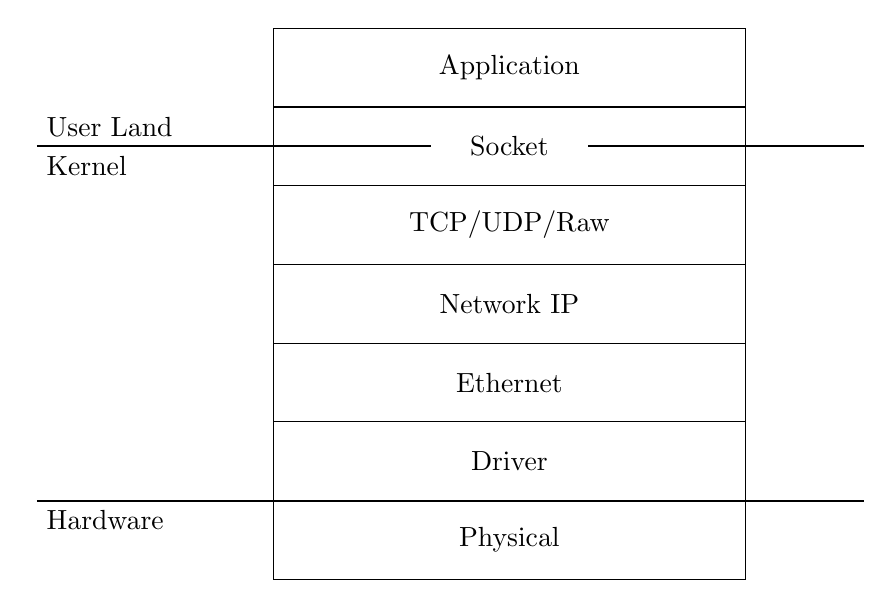
\begin{tikzpicture}
  \draw (-1,0) rectangle +(6,1) node(l1) [midway] {Physical};
  \draw (-1,1) rectangle +(6,1) node(l1) [midway] {Driver};
  \draw (-1,2) rectangle +(6,1) node(l2) [midway] {Ethernet};
  \draw (-1,3) rectangle +(6,1) node(l3) [midway] {Network IP};
  \draw (-1,4) rectangle +(6,1) node(l4) [midway] {TCP/UDP/Raw};
  \draw (-1,5) rectangle +(6,1) node(l5) [midway] {Socket};
  \draw (-1,6) rectangle +(6,1) node(l5) [midway] {Application};
  \draw[thick] (-4,5.5) node(context) {} -- +(5,0) +(7,0) -- +(10.5,0);
  \node [below right] at (context) {Kernel};
  \node [above right] at (context) {User Land};
  \draw[thick] (-4,1) node(hardware) {} -- +(10.5,0);
  \node [below right] at (hardware) {Hardware};
\end{tikzpicture}
\end{frame}

\section{Measurement}
\begin{frame}{Agenda}
\tableofcontents[currentsection]
\end{frame}

\subsection{Protocol Statistics Counter}
\begin{frame}[fragile]{Protocol Statistics Counter}
netstat -ss
\scriptsize
\begin{verbatim}
ip:
    2208239 total packets received
    2204405 packets for this host
    3717 packets for unknown/unsupported protocol
    101 packets not forwardable
tcp:
    1542163 packets sent
        616615 data packets (165690394 bytes)
        333 data packets (296898 bytes) retransmitted
        740242 ack-only packets (646590 delayed)
        153288 window update packets
\end{verbatim}
\end{frame}

\subsection{pf States}
\begin{frame}[fragile]{pf State}
pfctl -ss
\scriptsize
\begin{verbatim}
em0 tcp 80.154.94.48:22 <- 84.191.39.187:60436
       ESTABLISHED:ESTABLISHED
em0 tcp 192.168.0.31:22 (80.154.94.48:10031) <- 80.154.94.10:19890
       ESTABLISHED:ESTABLISHED
em1 tcp 80.154.94.10:19890 -> 192.168.0.31:22
       ESTABLISHED:ESTABLISHED
em0 tcp 192.168.0.31:443 (80.154.94.48:443) <- 193.30.66.53:51727
       CLOSING:ESTABLISHED
\end{verbatim}
\end{frame}

\subsection{Network Sockets}
\begin{frame}[fragile]{Network Sockets}
netstat -an
\scriptsize
\begin{verbatim}
Active Internet connections (including servers)
Proto   Recv-Q Send-Q  Local Address   Foreign Address  TCP-State
tcp          0      0  10.0.1.37.22    10.0.1.2.30176   ESTABLISHED
tcp          0   1144  10.0.1.37.22    10.0.1.1.27069   ESTABLISHED
tcp          0     44  10.0.1.37.22    10.0.1.2.49002   ESTABLISHED
tcp          0      0  *.22            *.*              LISTEN
Active Internet connections (including servers)
Proto   Recv-Q Send-Q  Local Address   Foreign Address
udp          0      0  10.0.1.37.7040  10.0.1.1.123
udp          0      0  10.0.1.37.161   *.*
udp          0      0  *.*             *.*
\end{verbatim}
\end{frame}

\subsection{Tcpdump Traffic}
\begin{frame}[fragile]{Tcpdump Traffic}
tcpdump -ni enc0 -v
\scriptsize
\begin{verbatim}
18:45:13.665393 (unprotected): SPI 0x00006861:
  fdd7:e83e:66bc:100::17 > fdd7:e83e:66bc:100::70:
  10.188.168.17 > 10.188.175.72:
  icmp: echo request
  (id:c52b seq:0) (ttl 255, id 8945, len 1028) (len 1028, hlim 64)
18:45:13.665849 (unprotected): SPI 0x00006862:
  fdd7:e83e:66bc:100::70 > fdd7:e83e:66bc:100::17:
  10.188.175.72 > 10.188.168.17:
  icmp: echo reply
  (id:c52b seq:0) (ttl 253, id 7503, len 1028) (len 1028, hlim 64)
\end{verbatim}
\end{frame}

\section{Packet Queues}
\begin{frame}{Agenda}
\tableofcontents[currentsection]
\end{frame}

\subsection{Input Queues}
\begin{frame}{Input Queues}
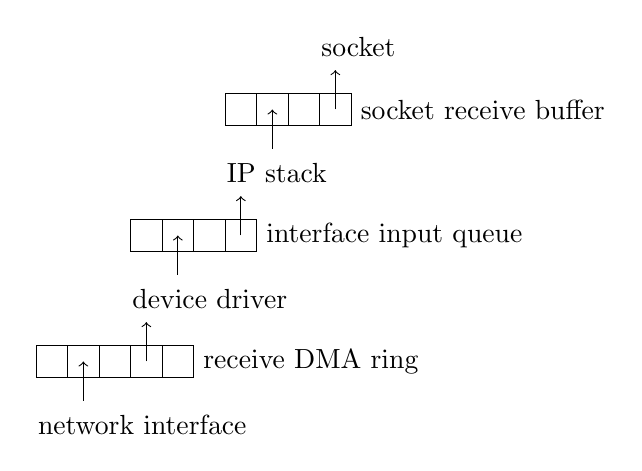
\begin{tikzpicture}
  \draw (0,0)
    node (ni) [right] {network interface} ++(.1,.6)
    rectangle ++(.4,.4) rectangle ++(.4,-.4)
    rectangle ++(.4,.4) rectangle ++(.4,-.4)
    rectangle ++(.4,.4) ++(0,-.2)
    node (rx) [right] {receive DMA ring} ++(-.5-1*.4,.8)
    node (dd) [right] {device driver} ++(.1,.6)
    rectangle ++(.4,.4) rectangle ++(.4,-.4)
    rectangle ++(.4,.4) rectangle ++(.4,-.4) ++(0,.2)
    node (iq) [right] {interface input queue} ++(-.5,.8)
    node (is) [right] {IP stack} ++(.1,.6)
    rectangle ++(.4,.4) rectangle ++(.4,-.4)
    rectangle ++(.4,.4) rectangle ++(.4,-.4) ++(0,.2)
    node (rb) [right] {socket receive buffer} ++(-.5,.8)
    node (so) [right] {socket}
    ;
  \path (node cs:name=ni,anchor=west) +(.3+1*.4,.3) coordinate (nio) {};
  \path (node cs:name=rx,anchor=west) +(-.2-3*.4,0) coordinate (rxi) {};
  \draw[->] (nio) -- (rxi);
  \path (node cs:name=rx,anchor=west) +(-.2-1*.4,0) coordinate (rxo) {};
  \path (node cs:name=dd,anchor=west) +(.3,-.3) coordinate (ddi) {};
  \draw[->] (rxo) -- (ddi);
  \path (node cs:name=dd,anchor=west) +(.3+1*.4,.3) coordinate (ddo) {};
  \path (node cs:name=iq,anchor=west) +(-.2-2*.4,0) coordinate (iqi) {};
  \draw[->] (ddo) -- (iqi);
  \path (node cs:name=iq,anchor=west) +(-.2,0) coordinate (iqo) {};
  \path (node cs:name=is,anchor=west) +(.3,-.3) coordinate (isi) {};
  \draw[->] (iqo) -- (isi);
  \path (node cs:name=is,anchor=west) +(.3+1*.4,.3) coordinate (iso) {};
  \path (node cs:name=rb,anchor=west) +(-.2-2*.4,0) coordinate (rbi) {};
  \draw[->] (iso) -- (rbi);
  \path (node cs:name=rb,anchor=west) +(-.2,0) coordinate (rbo) {};
  \path (node cs:name=so,anchor=west) +(.3,-.3) coordinate (soi) {};
  \draw[->] (rbo) -- (soi);
\end{tikzpicture}
\end{frame}

\subsection{Output Queues}
\begin{frame}{Output Queues}
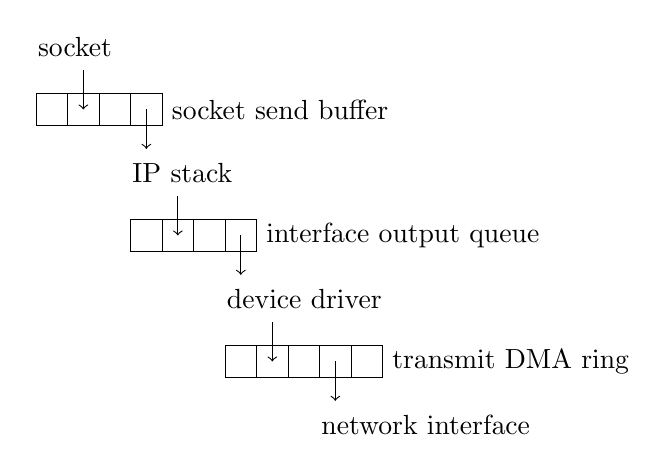
\begin{tikzpicture}
  \draw (0,0)
    node (so) [right] {socket} ++(.1,-.6)
    rectangle ++(.4,-.4) rectangle ++(.4,.4)
    rectangle ++(.4,-.4) rectangle ++(.4,.4) ++(0,-.2)
    node (sb) [right] {socket send buffer} ++(-.5,-.8)
    node (is) [right] {IP stack} ++(.1,-.6)
    rectangle ++(.4,-.4) rectangle ++(.4,.4)
    rectangle ++(.4,-.4) rectangle ++(.4,.4) ++(0,-.2)
    node (oq) [right] {interface output queue} ++(-.5,-.8)
    node (dd) [right] {device driver} ++(.1,-.6)
    rectangle ++(.4,-.4) rectangle ++(.4,.4)
    rectangle ++(.4,-.4) rectangle ++(.4,.4)
    rectangle ++(.4,-.4) ++(0,.2)
    node (tx) [right] {transmit DMA ring} ++(-.5-1*.4,-.8)
    node (ni) [right] {network interface}
    ;
  \path (node cs:name=so,anchor=west) +(.3+1*.4,-.3) coordinate (soo) {};
  \path (node cs:name=sb,anchor=west) +(-.2-2*.4,0) coordinate (sbi) {};
  \draw[->] (soo) -- (sbi);
  \path (node cs:name=sb,anchor=west) +(-.2,0) coordinate (sbo) {};
  \path (node cs:name=is,anchor=west) +(.3,.3) coordinate (isi) {};
  \draw[->] (sbo) -- (isi);
  \path (node cs:name=is,anchor=west) +(.3+1*.4,-.3) coordinate (iso) {};
  \path (node cs:name=oq,anchor=west) +(-.2-2*.4,0) coordinate (oqi) {};
  \draw[->] (iso) -- (oqi);
  \path (node cs:name=oq,anchor=west) +(-.2,0) coordinate (oqo) {};
  \path (node cs:name=dd,anchor=west) +(.3,.3) coordinate (ddi) {};
  \draw[->] (oqo) -- (ddi);
  \path (node cs:name=dd,anchor=west) +(.3+1*.4,-.3) coordinate (ddo) {};
  \path (node cs:name=tx,anchor=west) +(-.2-3*.4,0) coordinate (txi) {};
  \draw[->] (ddo) -- (txi);
  \path (node cs:name=tx,anchor=west) +(-.2-1*.4,0) coordinate (txo) {};
  \path (node cs:name=ni,anchor=west) +(.3,.3) coordinate (nii) {};
  \draw[->] (txo) -- (nii);
\end{tikzpicture}
\end{frame}

\subsection{Socket Buffer Recv-Q Send-Q}
\begin{frame}[fragile]{Socket Buffer Recv-Q Send-Q}
\begin{framed}
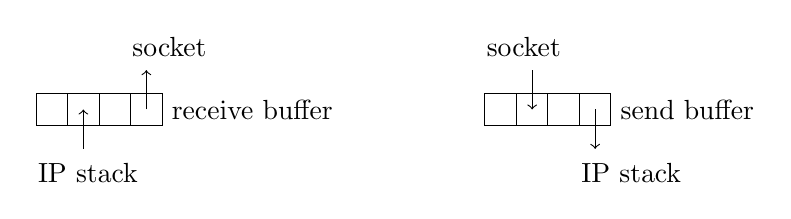
\begin{tikzpicture}
  \draw (0,0)
    node (iis) [right] {IP stack} ++(.1,.6)
    rectangle ++(.4,.4) rectangle ++(.4,-.4)
    rectangle ++(.4,.4) rectangle ++(.4,-.4) ++(0,.2)
    node (irb) [right] {receive buffer} ++(-.5,.8)
    node (iso) [right] {socket} ++(4.5,0)

    node (oso) [right] {socket} ++(.1,-.6)
    rectangle ++(.4,-.4) rectangle ++(.4,.4)
    rectangle ++(.4,-.4) rectangle ++(.4,.4) ++(0,-.2)
    node (osb) [right] {send buffer} ++(-.5,-.8)
    node (ois) [right] {IP stack}
    ;
  \path (node cs:name=iis,anchor=west) +(.3+1*.4,.3) coordinate (iiso) {};
  \path (node cs:name=irb,anchor=west) +(-.2-2*.4,0) coordinate (irbi) {};
  \draw[->] (iiso) -- (irbi);
  \path (node cs:name=irb,anchor=west) +(-.2,0) coordinate (irbo) {};
  \path (node cs:name=iso,anchor=west) +(.3,-.3) coordinate (isoi) {};
  \draw[->] (irbo) -- (isoi);
  \path (node cs:name=oso,anchor=west) +(.3+1*.4,-.3) coordinate (osoo) {};
  \path (node cs:name=osb,anchor=west) +(-.2-2*.4,0) coordinate (osbi) {};
  \draw[->] (osoo) -- (osbi);
  \path (node cs:name=osb,anchor=west) +(-.2,0) coordinate (osbo) {};
  \path (node cs:name=ois,anchor=west) +(.3,.3) coordinate (oisi) {};
  \draw[->] (osbo) -- (oisi);
\end{tikzpicture}
\end{framed}
netstat -n -p tcp
\scriptsize
\begin{verbatim}
Active Internet connections (including servers)
Proto  Recv-Q Send-Q  Local Address     Foreign Address   TCP-State
tcp     65160      0  10.10.11.2.35477  10.10.11.1.41996  ESTABLISHED
tcp         0 131732  10.10.12.3.44648  10.10.12.4.12345  ESTABLISHED
\end{verbatim}
\end{frame}

\subsection{Interface Queue qdrops}
\begin{frame}[fragile]{Interface Queue qdrops}
\begin{framed}
\begin{tikzpicture}
  \draw (0,0)
    node (idd) [right] {device driver} ++(.1,.6)
    rectangle ++(.4,.4) rectangle ++(.4,-.4)
    rectangle ++(.4,.4) rectangle ++(.4,-.4) ++(0,.2)
    node (iq) [right] {input queue} ++(-.5,.8)
    node (iis) [right] {IP stack} ++(4,0)
    node (ois) [right] {IP stack} ++(.1,-.6)
    rectangle ++(.4,-.4) rectangle ++(.4,.4)
    rectangle ++(.4,-.4) rectangle ++(.4,.4) ++(0,-.2)
    node (oq) [right] {output queue} ++(-.5,-.8)
    node (odd) [right] {device driver}
    ;
  \path (node cs:name=idd,anchor=west) +(.3+1*.4,.3) coordinate (iddo) {};
  \path (node cs:name=iq,anchor=west) +(-.2-2*.4,0) coordinate (iqi) {};
  \draw[->] (iiso) -- (iqi);
  \path (node cs:name=iq,anchor=west) +(-.2,0) coordinate (iqo) {};
  \path (node cs:name=iis,anchor=west) +(.3,-.3) coordinate (iisi) {};
  \draw[->] (iqo) -- (iisi);
  \path (node cs:name=ois,anchor=west) +(.3+1*.4,-.3) coordinate (oiso) {};
  \path (node cs:name=oq,anchor=west) +(-.2-2*.4,0) coordinate (oqi) {};
  \draw[->] (oiso) -- (oqi);
  \path (node cs:name=oq,anchor=west) +(-.2,0) coordinate (oqo) {};
  \path (node cs:name=odd,anchor=west) +(.3,.3) coordinate (oddi) {};
  \draw[->] (oqo) -- (oddi);
\end{tikzpicture}
\end{framed}
kstat
\\
\vspace{.2cm}
\scriptsize
\begin{tabular}{ll}
  \begin{minipage}{4.8cm}
  \begin{verbatim}
ix0:0:rxq:0
     packets: 158069114 packets
       bytes: 300328302395 bytes
      qdrops: 7902615 packets
        qlen: 0 packets
    enqueues: 6947931
    dequeues: 5729695
  \end{verbatim}
  \end{minipage}
  &
  \begin{minipage}{4.8cm}
  \begin{verbatim}
ix0:0:txq:0
     packets: 11094621 packets
       bytes: 894601044 bytes
      qdrops: 0 packets
        qlen: 0 packets
     maxqlen: 255 packets

  \end{verbatim}
  \end{minipage}
  \\
\end{tabular}
\end{frame}

\subsection{Device Driver OACTIVE}
\begin{frame}[fragile]{Device Driver OACTIVE}
\begin{framed}
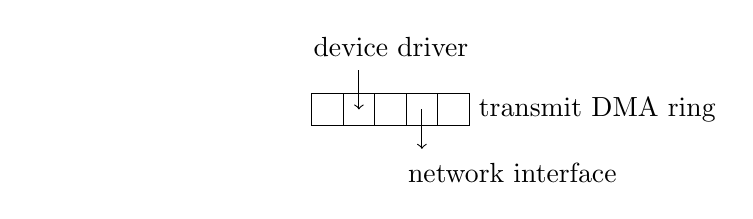
\begin{tikzpicture}
  \draw (0,0) ++(3.5,0)
    node (dd) [right] {device driver} ++(.1,-.6)
    rectangle ++(.4,-.4) rectangle ++(.4,.4)
    rectangle ++(.4,-.4) rectangle ++(.4,.4)
    rectangle ++(.4,-.4) ++(0,.2)
    node (tx) [right] {transmit DMA ring} ++(-.5-1*.4,-.8)
    node (ni) [right] {network interface}
    ;
  \path (node cs:name=dd,anchor=west) +(.3+1*.4,-.3) coordinate (ddo) {};
  \path (node cs:name=tx,anchor=west) +(-.2-3*.4,0) coordinate (txi) {};
  \draw[->] (ddo) -- (txi);
  \path (node cs:name=tx,anchor=west) +(-.2-1*.4,0) coordinate (txo) {};
  \path (node cs:name=ni,anchor=west) +(.3,.3) coordinate (nii) {};
  \draw[->] (txo) -- (nii);
\end{tikzpicture}
\end{framed}
ifconfig em1
\scriptsize
\begin{verbatim}
em1: flags=8c43<UP,BROADCAST,RUNNING,OACTIVE,SIMPLEX,MULTICAST> mtu 1500
        lladdr 0c:c4:7a:78:f3:55
        description: Intel I210
        index 6 priority 0 llprio 3
        media: Ethernet autoselect (1000baseT full-duplex)
        status: active
        inet 10.10.12.3 netmask 0xffffff00 broadcast 10.10.12.255
\end{verbatim}
\end{frame}

\subsection{Transmit Rings oactives}
\begin{frame}[fragile]{Transmit Rings oactives}
dmesg
\scriptsize
\begin{verbatim}
ix1 at pci1 dev 0 function 1 "Intel X550T" rev 0x01, msix,
  4 queues, address a0:36:9f:e0:52:55
\end{verbatim}
\normalsize
kstat txq
\\
\vspace{.3cm}
\scriptsize
\begin{tabular}{ll}
  \begin{minipage}{4.8cm}
  \begin{verbatim}
ix1:0:txq:0
        qlen: 90 packets
     maxqlen: 255 packets
     oactive: true
    oactives: 1919595
  \end{verbatim}
  \end{minipage}
  &
  \begin{minipage}{4.8cm}
  \begin{verbatim}
ix1:0:txq:1
        qlen: 141 packets
     maxqlen: 255 packets
     oactive: true
    oactives: 2251633
  \end{verbatim}
  \end{minipage}
  \\
  \begin{minipage}{4.8cm}
  \begin{verbatim}
ix1:0:txq:2
        qlen: 6 packets
     maxqlen: 255 packets
     oactive: true
    oactives: 1788971
  \end{verbatim}
  \end{minipage}
  &
  \begin{minipage}{4.8cm}
  \begin{verbatim}
ix1:0:txq:3
        qlen: 55 packets
     maxqlen: 255 packets
     oactive: true
    oactives: 1925063
  \end{verbatim}
  \end{minipage}
  \\
\end{tabular}
\end{frame}

\section{IP Stack}
\begin{frame}{Agenda}
\tableofcontents[currentsection]
\end{frame}

\subsection{Protocol Stack}
\begin{frame}{Protocol Stack}
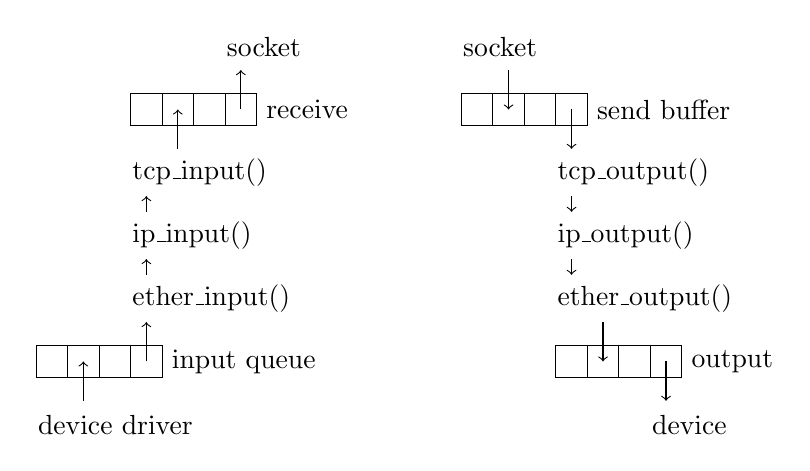
\begin{tikzpicture}
  \draw (0,0)
    node (idd) [right] {device driver} ++(.1,.6)
    rectangle ++(.4,.4) rectangle ++(.4,-.4)
    rectangle ++(.4,.4) rectangle ++(.4,-.4) ++(0,.2)
    node (iq) [right] {input queue} ++(-.5,.8)
    node (ei) [right] {ether\_input()} ++(0,.8)
    node (ii) [right] {ip\_input()} ++(0,.8)
    node (ti) [right] {tcp\_input()} ++(.1,.6)
    rectangle ++(.4,.4) rectangle ++(.4,-.4)
    rectangle ++(.4,.4) rectangle ++(.4,-.4) ++(0,.2)
    node (rb) [right] {receive} ++(-.5,.8)
    node (iso) [right] {socket} ++(3,0)

    node (oso) [right] {socket} ++(.1,-.6)
    rectangle ++(.4,-.4) rectangle ++(.4,.4)
    rectangle ++(.4,-.4) rectangle ++(.4,.4) ++(0,-.2)
    node (sb) [right] {send buffer} ++(-.5,-.8)
    node (to) [right] {tcp\_output()} ++(0,-.8)
    node (io) [right] {ip\_output()} ++(0,-.8)
    node (eo) [right] {ether\_output()} ++(.1,-.6)
    rectangle ++(.4,-.4) rectangle ++(.4,.4)
    rectangle ++(.4,-.4) rectangle ++(.4,.4) ++(0,-.2)
    node (oq) [right] {output} ++(-.5,-.8)
    node (odd) [right] {device}
    ;
  \path (node cs:name=idd,anchor=west) +(.3+1*.4,.3) coordinate (iddo) {};
  \path (node cs:name=iq,anchor=west) +(-.2-2*.4,0) coordinate (iqi) {};
  \draw[->] (iddo) -- (iqi);
  \path (node cs:name=iq,anchor=west) +(-.2,0) coordinate (iqo) {};
  \path (node cs:name=ei,anchor=west) +(.3,-.3) coordinate (iei) {};
  \draw[->] (iqo) -- (iei);
  \path (node cs:name=ei,anchor=west) +(.3,.3) coordinate (eio) {};
  \path (node cs:name=ii,anchor=west) +(.3,-.3) coordinate (iii) {};
  \draw[->] (eio) -- (iii);
  \path (node cs:name=ii,anchor=west) +(.3,.3) coordinate (iio) {};
  \path (node cs:name=ti,anchor=west) +(.3,-.3) coordinate (tii) {};
  \draw[->] (iio) -- (tii);
  \path (node cs:name=ti,anchor=west) +(.3+1*.4,.3) coordinate (iti) {};
  \path (node cs:name=rb,anchor=west) +(-.2-2*.4,0) coordinate (rbi) {};
  \draw[->] (iti) -- (rbi);
  \path (node cs:name=rb,anchor=west) +(-.2,0) coordinate (rbo) {};
  \path (node cs:name=iso,anchor=west) +(.3,-.3) coordinate (isoi) {};
  \draw[->] (rbo) -- (isoi);

  \path (node cs:name=oso,anchor=west) +(.3+1*.4,-.3) coordinate (osoo) {};
  \path (node cs:name=sb,anchor=west) +(-.2-2*.4,0) coordinate (sbi) {};
  \draw[->] (osoo) -- (sbi);
  \path (node cs:name=sb,anchor=west) +(-.2,0) coordinate (sbo) {};
  \path (node cs:name=to,anchor=west) +(.3,.3) coordinate (toi) {};
  \draw[->] (sbo) -- (toi);
  \path (node cs:name=to,anchor=west) +(.3,-.3) coordinate (too) {};
  \path (node cs:name=io,anchor=west) +(.3,.3) coordinate (ioi) {};
  \draw[->] (too) -- (ioi);
  \path (node cs:name=io,anchor=west) +(.3,-.3) coordinate (ioo) {};
  \path (node cs:name=eo,anchor=west) +(.3,.3) coordinate (eoi) {};
  \draw[->] (ioo) -- (eoi);
  \path (node cs:name=eo,anchor=west) +(.3+1*.4,-.3) coordinate (eoo) {};
  \path (node cs:name=oq,anchor=west) +(-.2-2*.4,0) coordinate (oqi) {};
  \draw[->] (eoo) -- (oqi);
  \path (node cs:name=oq,anchor=west) +(-.2,0) coordinate (oqo) {};
  \path (node cs:name=odd,anchor=west) +(.3,.3) coordinate (oddi) {};
  \draw[->] (oqo) -- (oddi);
\end{tikzpicture}
\end{frame}

\subsection{IP Forwarding}
\begin{frame}{IP Forwarding}
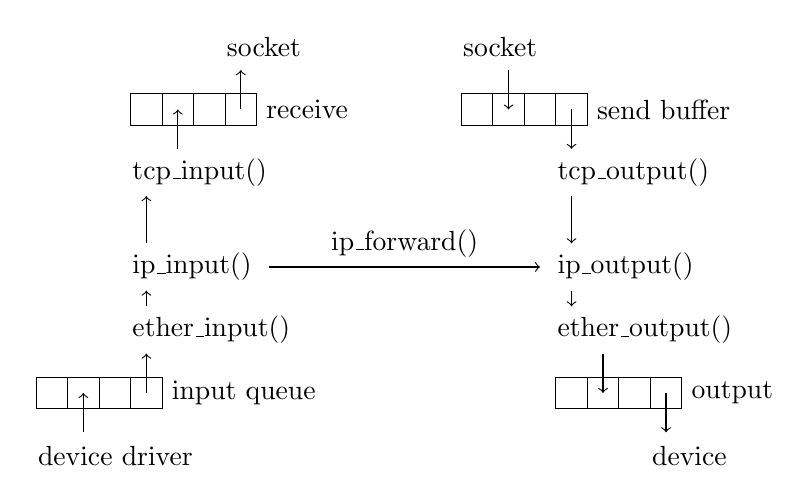
\begin{tikzpicture}
  \draw (0,0)
    node (idd) [right] {device driver} ++(.1,.6)
    rectangle ++(.4,.4) rectangle ++(.4,-.4)
    rectangle ++(.4,.4) rectangle ++(.4,-.4) ++(0,.2)
    node (iq) [right] {input queue} ++(-.5,.8)
    node (ei) [right] {ether\_input()} ++(0,.8)
    node (ii) [right] {ip\_input()} ++(0,1.2)
    node (ti) [right] {tcp\_input()} ++(.1,.6)
    rectangle ++(.4,.4) rectangle ++(.4,-.4)
    rectangle ++(.4,.4) rectangle ++(.4,-.4) ++(0,.2)
    node (rb) [right] {receive} ++(-.5,.8)
    node (iso) [right] {socket} ++(3,0)

    node (oso) [right] {socket} ++(.1,-.6)
    rectangle ++(.4,-.4) rectangle ++(.4,.4)
    rectangle ++(.4,-.4) rectangle ++(.4,.4) ++(0,-.2)
    node (sb) [right] {send buffer} ++(-.5,-.8)
    node (to) [right] {tcp\_output()} ++(0,-1.2)
    node (io) [right] {ip\_output()} ++(0,-.8)
    node (eo) [right] {ether\_output()} ++(.1,-.6)
    rectangle ++(.4,-.4) rectangle ++(.4,.4)
    rectangle ++(.4,-.4) rectangle ++(.4,.4) ++(0,-.2)
    node (oq) [right] {output} ++(-.5,-.8)
    node (odd) [right] {device}
    ;
  \path (node cs:name=idd,anchor=west) +(.3+1*.4,.3) coordinate (iddo) {};
  \path (node cs:name=iq,anchor=west) +(-.2-2*.4,0) coordinate (iqi) {};
  \draw[->] (iddo) -- (iqi);
  \path (node cs:name=iq,anchor=west) +(-.2,0) coordinate (iqo) {};
  \path (node cs:name=ei,anchor=west) +(.3,-.3) coordinate (iei) {};
  \draw[->] (iqo) -- (iei);
  \path (node cs:name=ei,anchor=west) +(.3,.3) coordinate (eio) {};
  \path (node cs:name=ii,anchor=west) +(.3,-.3) coordinate (iii) {};
  \draw[->] (eio) -- (iii);
  \path (node cs:name=ii,anchor=west) +(.3,.3) coordinate (iio) {};
  \path (node cs:name=ti,anchor=west) +(.3,-.3) coordinate (tii) {};
  \draw[->] (iio) -- (tii);
  \path (node cs:name=ti,anchor=west) +(.3+1*.4,.3) coordinate (iti) {};
  \path (node cs:name=rb,anchor=west) +(-.2-2*.4,0) coordinate (rbi) {};
  \draw[->] (iti) -- (rbi);
  \path (node cs:name=rb,anchor=west) +(-.2,0) coordinate (rbo) {};
  \path (node cs:name=iso,anchor=west) +(.3,-.3) coordinate (isoi) {};
  \draw[->] (rbo) -- (isoi);

  \path (node cs:name=oso,anchor=west) +(.3+1*.4,-.3) coordinate (osoo) {};
  \path (node cs:name=sb,anchor=west) +(-.2-2*.4,0) coordinate (sbi) {};
  \draw[->] (osoo) -- (sbi);
  \path (node cs:name=sb,anchor=west) +(-.2,0) coordinate (sbo) {};
  \path (node cs:name=to,anchor=west) +(.3,.3) coordinate (toi) {};
  \draw[->] (sbo) -- (toi);
  \path (node cs:name=to,anchor=west) +(.3,-.3) coordinate (too) {};
  \path (node cs:name=io,anchor=west) +(.3,.3) coordinate (ioi) {};
  \draw[->] (too) -- (ioi);
  \path (node cs:name=io,anchor=west) +(.3,-.3) coordinate (ioo) {};
  \path (node cs:name=eo,anchor=west) +(.3,.3) coordinate (eoi) {};
  \draw[->] (ioo) -- (eoi);
  \path (node cs:name=eo,anchor=west) +(.3+1*.4,-.3) coordinate (eoo) {};
  \path (node cs:name=oq,anchor=west) +(-.2-2*.4,0) coordinate (oqi) {};
  \draw[->] (eoo) -- (oqi);
  \path (node cs:name=oq,anchor=west) +(-.2,0) coordinate (oqo) {};
  \path (node cs:name=odd,anchor=west) +(.3,.3) coordinate (oddi) {};
  \draw[->] (oqo) -- (oddi);

  \path (node cs:name=ii,anchor=east) +(.1,0) coordinate (ifo) {};
  \path (node cs:name=io,anchor=west) +(-.1,0) coordinate (ifi) {};
  \draw[->] (ifo) -- (ifi) node [midway,above] {ip\_forward()};
\end{tikzpicture}
\end{frame}

\subsection{UDP}
\begin{frame}{UDP}
\begin{tikzpicture}
  \draw (0,0)
    node (idd) [right] {device driver} ++(.1,.6)
    rectangle ++(.4,.4) rectangle ++(.4,-.4)
    rectangle ++(.4,.4) rectangle ++(.4,-.4) ++(0,.2)
    node (iq) [right] {input queue} ++(-.5,.8)
    node (ei) [right] {ether\_input()} ++(0,.8)
    node (ii) [right] {ip\_input()} ++(0,1.2)
    node (ui) [right] {udp\_input()} ++(.1,.6)
    rectangle ++(.4,.4) rectangle ++(.4,-.4)
    rectangle ++(.4,.4) rectangle ++(.4,-.4) ++(0,.2)
    node (rb) [right] {receive buffer} ++(-.5,.8)
    node (iso) [right] {socket} ++(4,0)

    node (oso) [right] {socket} ++(0,-1.6)
    node (uo) [right] {udp\_output()} ++(0,-1.2)
    node (io) [right] {ip\_output()} ++(0,-.8)
    node (eo) [right] {ether\_output()} ++(.1,-.6)
    rectangle ++(.4,-.4) rectangle ++(.4,.4)
    rectangle ++(.4,-.4) rectangle ++(.4,.4) ++(0,-.2)
    node (oq) [right] {output} ++(-.5,-.8)
    node (odd) [right] {device}
    ;
  \path (node cs:name=idd,anchor=west) +(.3+1*.4,.3) coordinate (iddo) {};
  \path (node cs:name=iq,anchor=west) +(-.2-2*.4,0) coordinate (iqi) {};
  \draw[->] (iddo) -- (iqi);
  \path (node cs:name=iq,anchor=west) +(-.2,0) coordinate (iqo) {};
  \path (node cs:name=ei,anchor=west) +(.3,-.3) coordinate (iei) {};
  \draw[->] (iqo) -- (iei);
  \path (node cs:name=ei,anchor=west) +(.3,.3) coordinate (eio) {};
  \path (node cs:name=ii,anchor=west) +(.3,-.3) coordinate (iii) {};
  \draw[->] (eio) -- (iii);
  \path (node cs:name=ii,anchor=west) +(.3,.3) coordinate (iio) {};
  \path (node cs:name=ui,anchor=west) +(.3,-.3) coordinate (uii) {};
  \draw[->] (iio) -- (uii);
  \path (node cs:name=ti,anchor=west) +(.3+1*.4,.3) coordinate (iti) {};
  \path (node cs:name=rb,anchor=west) +(-.2-2*.4,0) coordinate (rbi) {};
  \draw[->] (iti) -- (rbi);
  \path (node cs:name=rb,anchor=west) +(-.2,0) coordinate (rbo) {};
  \path (node cs:name=iso,anchor=west) +(.3,-.3) coordinate (isoi) {};
  \draw[->] (rbo) -- (isoi);

  \path (node cs:name=oso,anchor=west) +(.3,-.3) coordinate (osoo) {};
  \path (node cs:name=uo,anchor=west) +(.3,.3) coordinate (uoi) {};
  \draw[->] (osoo) -- (uoi);
  \path (node cs:name=uo,anchor=west) +(.3,-.3) coordinate (uoo) {};
  \path (node cs:name=io,anchor=west) +(.3,.3) coordinate (ioi) {};
  \draw[->] (uoo) -- (ioi);
  \path (node cs:name=io,anchor=west) +(.3,-.3) coordinate (ioo) {};
  \path (node cs:name=eo,anchor=west) +(.3,.3) coordinate (eoi) {};
  \draw[->] (ioo) -- (eoi);
  \path (node cs:name=eo,anchor=west) +(.3+1*.4,-.3) coordinate (eoo) {};
  \path (node cs:name=oq,anchor=west) +(-.2-2*.4,0) coordinate (oqi) {};
  \draw[->] (eoo) -- (oqi);
  \path (node cs:name=oq,anchor=west) +(-.2,0) coordinate (oqo) {};
  \path (node cs:name=odd,anchor=west) +(.3,.3) coordinate (oddi) {};
  \draw[->] (oqo) -- (oddi);

  \path (node cs:name=ii,anchor=east) +(.1,0) coordinate (ifo) {};
  \path (node cs:name=io,anchor=west) +(-.1,0) coordinate (ifi) {};
  \draw[->] (ifo) -- (ifi) node [midway,above] {ip\_forward()};
\end{tikzpicture}
\end{frame}

\subsection{IPv6}
\begin{frame}{IPv6}
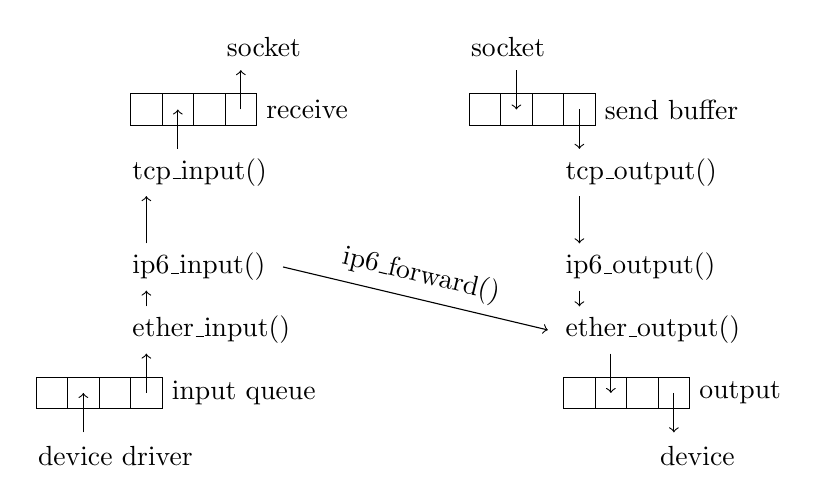
\begin{tikzpicture}
  \draw (0,0)
    node (idd) [right] {device driver} ++(.1,.6)
    rectangle ++(.4,.4) rectangle ++(.4,-.4)
    rectangle ++(.4,.4) rectangle ++(.4,-.4) ++(0,.2)
    node (iq) [right] {input queue} ++(-.5,.8)
    node (ei) [right] {ether\_input()} ++(0,.8)
    node (ii) [right] {ip6\_input()} ++(0,1.2)
    node (ti) [right] {tcp\_input()} ++(.1,.6)
    rectangle ++(.4,.4) rectangle ++(.4,-.4)
    rectangle ++(.4,.4) rectangle ++(.4,-.4) ++(0,.2)
    node (rb) [right] {receive} ++(-.5,.8)
    node (iso) [right] {socket} ++(3.1,0)

    node (oso) [right] {socket} ++(.1,-.6)
    rectangle ++(.4,-.4) rectangle ++(.4,.4)
    rectangle ++(.4,-.4) rectangle ++(.4,.4) ++(0,-.2)
    node (sb) [right] {send buffer} ++(-.5,-.8)
    node (to) [right] {tcp\_output()} ++(0,-1.2)
    node (io) [right] {ip6\_output()} ++(0,-.8)
    node (eo) [right] {ether\_output()} ++(.1,-.6)
    rectangle ++(.4,-.4) rectangle ++(.4,.4)
    rectangle ++(.4,-.4) rectangle ++(.4,.4) ++(0,-.2)
    node (oq) [right] {output} ++(-.5,-.8)
    node (odd) [right] {device}
    ;
  \path (node cs:name=idd,anchor=west) +(.3+1*.4,.3) coordinate (iddo) {};
  \path (node cs:name=iq,anchor=west) +(-.2-2*.4,0) coordinate (iqi) {};
  \draw[->] (iddo) -- (iqi);
  \path (node cs:name=iq,anchor=west) +(-.2,0) coordinate (iqo) {};
  \path (node cs:name=ei,anchor=west) +(.3,-.3) coordinate (iei) {};
  \draw[->] (iqo) -- (iei);
  \path (node cs:name=ei,anchor=west) +(.3,.3) coordinate (eio) {};
  \path (node cs:name=ii,anchor=west) +(.3,-.3) coordinate (iii) {};
  \draw[->] (eio) -- (iii);
  \path (node cs:name=ii,anchor=west) +(.3,.3) coordinate (iio) {};
  \path (node cs:name=ti,anchor=west) +(.3,-.3) coordinate (tii) {};
  \draw[->] (iio) -- (tii);
  \path (node cs:name=ti,anchor=west) +(.3+1*.4,.3) coordinate (iti) {};
  \path (node cs:name=rb,anchor=west) +(-.2-2*.4,0) coordinate (rbi) {};
  \draw[->] (iti) -- (rbi);
  \path (node cs:name=rb,anchor=west) +(-.2,0) coordinate (rbo) {};
  \path (node cs:name=iso,anchor=west) +(.3,-.3) coordinate (isoi) {};
  \draw[->] (rbo) -- (isoi);

  \path (node cs:name=oso,anchor=west) +(.3+1*.4,-.3) coordinate (osoo) {};
  \path (node cs:name=sb,anchor=west) +(-.2-2*.4,0) coordinate (sbi) {};
  \draw[->] (osoo) -- (sbi);
  \path (node cs:name=sb,anchor=west) +(-.2,0) coordinate (sbo) {};
  \path (node cs:name=to,anchor=west) +(.3,.3) coordinate (toi) {};
  \draw[->] (sbo) -- (toi);
  \path (node cs:name=to,anchor=west) +(.3,-.3) coordinate (too) {};
  \path (node cs:name=io,anchor=west) +(.3,.3) coordinate (ioi) {};
  \draw[->] (too) -- (ioi);
  \path (node cs:name=io,anchor=west) +(.3,-.3) coordinate (ioo) {};
  \path (node cs:name=eo,anchor=west) +(.3,.3) coordinate (eoi) {};
  \draw[->] (ioo) -- (eoi);
  \path (node cs:name=eo,anchor=west) +(.3+1*.4,-.3) coordinate (eoo) {};
  \path (node cs:name=oq,anchor=west) +(-.2-2*.4,0) coordinate (oqi) {};
  \draw[->] (eoo) -- (oqi);
  \path (node cs:name=oq,anchor=west) +(-.2,0) coordinate (oqo) {};
  \path (node cs:name=odd,anchor=west) +(.3,.3) coordinate (oddi) {};
  \draw[->] (oqo) -- (oddi);

  \path (node cs:name=ii,anchor=east) +(.1,0) coordinate (ifo) {};
  \path (node cs:name=eo,anchor=west) +(-.1,0) coordinate (ifi) {};
  \draw[->] (ifo) -- (ifi) node [midway,above,sloped] {ip6\_forward()};
\end{tikzpicture}
\end{frame}

\subsection{Netstat Counter}
\begin{frame}[fragile]{Netstat Counter}
netstat -ss
\scriptsize
\begin{verbatim}
ip:
        393285673 total packets received
        246049103 packets for this host
        126364372 packets forwarded
        242653961 packets sent from this host
tcp:
        86520236 packets sent
        123883097 packets received
udp:
        400260722 datagrams received
        82147309 dropped due to full socket buffers
        318113273 delivered
        396391499 datagrams output
ip6:
        434697159 total packets received
        278214439 packets for this host
        146543897 packets forwarded
        240423068 packets sent from this host
\end{verbatim}
\end{frame}

\subsection{pf Test}
\begin{frame}{pf Test}
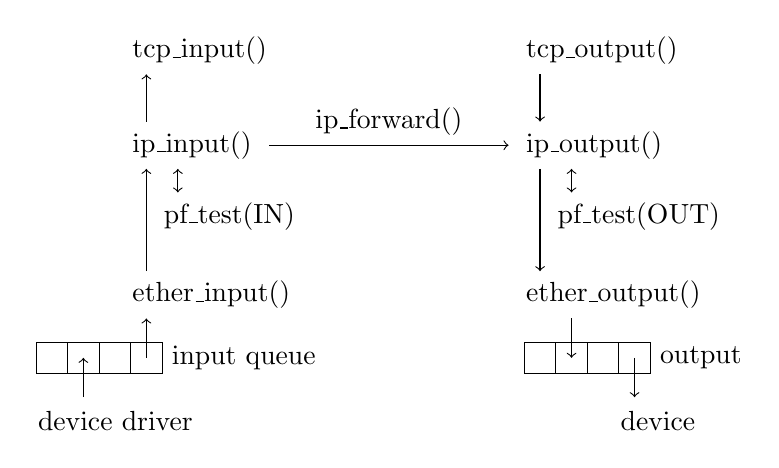
\begin{tikzpicture}
  \draw (0,0)
    node (idd) [right] {device driver} ++(.1,.6)
    rectangle ++(.4,.4) rectangle ++(.4,-.4)
    rectangle ++(.4,.4) rectangle ++(.4,-.4) ++(0,.2)
    node (iq) [right] {input queue} ++(-.5,.8)
    node (ei) [right] {ether\_input()} ++(0.4,1)
    node (pi) [right] {pf\_test(IN)} ++(-0.4,.9)
    node (ii) [right] {ip\_input()} ++(0,1.2)
    node (ti) [right] {tcp\_input()} ++(5,0)

    node (to) [right] {tcp\_output()} ++(0,-1.2)
    node (io) [right] {ip\_output()} ++(0.4,-.9)
    node (po) [right] {pf\_test(OUT)} ++(-0.4,-1)
    node (eo) [right] {ether\_output()} ++(.1,-.6)
    rectangle ++(.4,-.4) rectangle ++(.4,.4)
    rectangle ++(.4,-.4) rectangle ++(.4,.4) ++(0,-.2)
    node (oq) [right] {output} ++(-.5,-.8)
    node (odd) [right] {device}
    ;
  \path (node cs:name=idd,anchor=west) +(.3+1*.4,.3) coordinate (iddo) {};
  \path (node cs:name=iq,anchor=west) +(-.2-2*.4,0) coordinate (iqi) {};
  \draw[->] (iddo) -- (iqi);
  \path (node cs:name=iq,anchor=west) +(-.2,0) coordinate (iqo) {};
  \path (node cs:name=ei,anchor=west) +(.3,-.3) coordinate (iei) {};
  \draw[->] (iqo) -- (iei);
  \path (node cs:name=ei,anchor=west) +(.3,.3) coordinate (eio) {};
  \path (node cs:name=ii,anchor=west) +(.3,-.3) coordinate (iii) {};
  \draw[->] (eio) -- (iii);
  \path (node cs:name=ii,anchor=west) +(.3,.3) coordinate (iio) {};
  \path (node cs:name=ti,anchor=west) +(.3,-.3) coordinate (tii) {};
  \draw[->] (iio) -- (tii);
  \path (node cs:name=ii,anchor=west) +(.7,-.3) coordinate (iip) {};
  \path (node cs:name=pi,anchor=west) +(.3,.3) coordinate (pii) {};
  \draw[<->] (iip) -- (pii);

  \path (node cs:name=to,anchor=west) +(.3,-.3) coordinate (too) {};
  \path (node cs:name=io,anchor=west) +(.3,.3) coordinate (ioi) {};
  \draw[->] (too) -- (ioi);
  \path (node cs:name=io,anchor=west) +(.3,-.3) coordinate (ioo) {};
  \path (node cs:name=eo,anchor=west) +(.3,.3) coordinate (eoi) {};
  \draw[->] (ioo) -- (eoi);
  \path (node cs:name=eo,anchor=west) +(.3+1*.4,-.3) coordinate (eoo) {};
  \path (node cs:name=oq,anchor=west) +(-.2-2*.4,0) coordinate (oqi) {};
  \draw[->] (eoo) -- (oqi);
  \path (node cs:name=oq,anchor=west) +(-.2,0) coordinate (oqo) {};
  \path (node cs:name=odd,anchor=west) +(.3,.3) coordinate (oddi) {};
  \draw[->] (oqo) -- (oddi);
  \path (node cs:name=io,anchor=west) +(.7,-.3) coordinate (iop) {};
  \path (node cs:name=po,anchor=west) +(.3,.3) coordinate (poi) {};
  \draw[<->] (iop) -- (poi);

  \path (node cs:name=ii,anchor=east) +(.1,0) coordinate (ifo) {};
  \path (node cs:name=io,anchor=west) +(-.1,0) coordinate (ifi) {};
  \draw[->] (ifo) -- (ifi) node [midway,above] {ip\_forward()};
\end{tikzpicture}
\end{frame}

\subsection{pf IPv6}
\begin{frame}{pf IPv6}
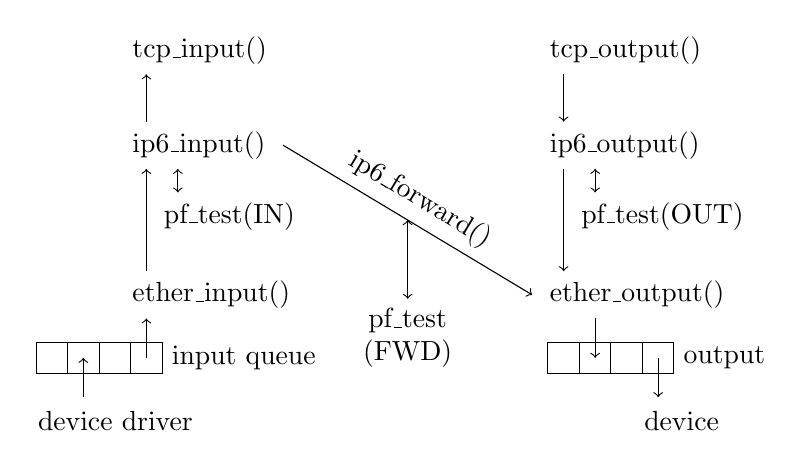
\begin{tikzpicture}
  \draw (0,0)
    node (idd) [right] {device driver} ++(.1,.6)
    rectangle ++(.4,.4) rectangle ++(.4,-.4)
    rectangle ++(.4,.4) rectangle ++(.4,-.4) ++(0,.2)
    node (iq) [right] {input queue} ++(-.5,.8)
    node (ei) [right] {ether\_input()} ++(0.4,1)
    node (pi) [right] {pf\_test(IN)} ++(-0.4,.9)
    node (ii) [right] {ip6\_input()} ++(0,1.2)
    node (ti) [right] {tcp\_input()} ++(5.3,0)

    node (to) [right] {tcp\_output()} ++(0,-1.2)
    node (io) [right] {ip6\_output()} ++(0.4,-.9)
    node (po) [right] {pf\_test(OUT)} ++(-0.4,-1)
    node (eo) [right] {ether\_output()} ++(.1,-.6)
    rectangle ++(.4,-.4) rectangle ++(.4,.4)
    rectangle ++(.4,-.4) rectangle ++(.4,.4) ++(0,-.2)
    node (oq) [right] {output} ++(-.5,-.8)
    node (odd) [right] {device}
    ;
  \path (node cs:name=idd,anchor=west) +(.3+1*.4,.3) coordinate (iddo) {};
  \path (node cs:name=iq,anchor=west) +(-.2-2*.4,0) coordinate (iqi) {};
  \draw[->] (iddo) -- (iqi);
  \path (node cs:name=iq,anchor=west) +(-.2,0) coordinate (iqo) {};
  \path (node cs:name=ei,anchor=west) +(.3,-.3) coordinate (iei) {};
  \draw[->] (iqo) -- (iei);
  \path (node cs:name=ei,anchor=west) +(.3,.3) coordinate (eio) {};
  \path (node cs:name=ii,anchor=west) +(.3,-.3) coordinate (iii) {};
  \draw[->] (eio) -- (iii);
  \path (node cs:name=ii,anchor=west) +(.3,.3) coordinate (iio) {};
  \path (node cs:name=ti,anchor=west) +(.3,-.3) coordinate (tii) {};
  \draw[->] (iio) -- (tii);
  \path (node cs:name=ii,anchor=west) +(.7,-.3) coordinate (iip) {};
  \path (node cs:name=pi,anchor=west) +(.3,.3) coordinate (pii) {};
  \draw[<->] (iip) -- (pii);

  \path (node cs:name=to,anchor=west) +(.3,-.3) coordinate (too) {};
  \path (node cs:name=io,anchor=west) +(.3,.3) coordinate (ioi) {};
  \draw[->] (too) -- (ioi);
  \path (node cs:name=io,anchor=west) +(.3,-.3) coordinate (ioo) {};
  \path (node cs:name=eo,anchor=west) +(.3,.3) coordinate (eoi) {};
  \draw[->] (ioo) -- (eoi);
  \path (node cs:name=eo,anchor=west) +(.3+1*.4,-.3) coordinate (eoo) {};
  \path (node cs:name=oq,anchor=west) +(-.2-2*.4,0) coordinate (oqi) {};
  \draw[->] (eoo) -- (oqi);
  \path (node cs:name=oq,anchor=west) +(-.2,0) coordinate (oqo) {};
  \path (node cs:name=odd,anchor=west) +(.3,.3) coordinate (oddi) {};
  \draw[->] (oqo) -- (oddi);
  \path (node cs:name=io,anchor=west) +(.7,-.3) coordinate (iop) {};
  \path (node cs:name=po,anchor=west) +(.3,.3) coordinate (poi) {};
  \draw[<->] (iop) -- (poi);

  \path (node cs:name=ii,anchor=east) +(.1,0) coordinate (ifo) {};
  \path (node cs:name=eo,anchor=west) +(-.1,0) coordinate (ifi) {};
  \draw[->] (ifo) -- (ifi) node (if) [midway,above,sloped] {ip6\_forward()};
  \draw[<->] (node cs:name=if,anchor=south) -- +(0,-1)
    node (pf) [below,align=center] {pf\_test\\ (FWD)};
\end{tikzpicture}
\end{frame}

\subsection{pf Rules}
\begin{frame}[fragile]{pf Rules}
pfctl -sr
\scriptsize
\begin{verbatim}
block return all
pass all flags S/SA
block return in on ! lo0 proto tcp from any to any port 6000:6010
block return out log proto tcp all user = 55
block return out log proto udp all user = 55
\end{verbatim}
\end{frame}

\section{Pseudo Devices}
\begin{frame}{Agenda}
\tableofcontents[currentsection]
\end{frame}

\subsection{Create Device}
\begin{frame}[fragile]{Create Device}
ifconfig -C
\scriptsize
\begin{verbatim}
aggr bpe bridge carp egre enc eoip etherip gif gre lo mgre mpe mpip
mpw nvgre pair pflog pflow pfsync ppp pppoe rport sec svlan tap
tpmr trunk tun veb vether vlan vport vxlan wg
\end{verbatim}
\normalsize
ifconfig vlan0 create vnetid 42 parent em0 up
\scriptsize
\begin{verbatim}
vlan0: flags=8843<UP,BROADCAST,RUNNING,SIMPLEX,MULTICAST> mtu 1500
        lladdr 0c:c4:7a:78:f3:54
        index 22 priority 0 llprio 3
        encap: vnetid 42 parent em0 txprio packet rxprio outer
        groups: vlan
        media: Ethernet autoselect (1000baseT full-duplex)
        status: active
\end{verbatim}
\end{frame}

\subsection{Hardware Receive and Tcpdump}
\begin{frame}{Hardware Receive and Tcpdump}
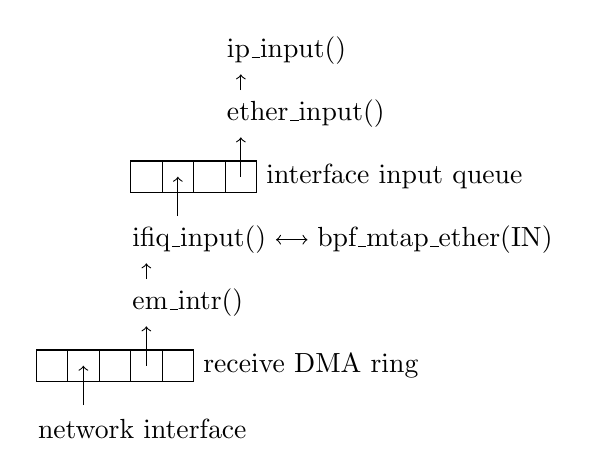
\begin{tikzpicture}
  \draw (0,0)
    node (ni) [right] {network interface} ++(.1,.6)
    rectangle ++(.4,.4) rectangle ++(.4,-.4)
    rectangle ++(.4,.4) rectangle ++(.4,-.4)
    rectangle ++(.4,.4) ++(0,-.2)
    node (rx) [right] {receive DMA ring} ++(-.5-1*.4,.8)
    node (em) [right] {em\_intr()} ++(0,.8)
    node (fq) [right] {ifiq\_input()} ++(.1,.6)
    rectangle ++(.4,.4) rectangle ++(.4,-.4)
    rectangle ++(.4,.4) rectangle ++(.4,-.4) ++(0,.2)
    node (iq) [right] {interface input queue} ++(-.5,.8)
    node (ei) [right] {ether\_input()} ++(0,.8)
    node (ii) [right] {ip\_input()}
    ;
  \path (node cs:name=ni,anchor=west) +(.3+1*.4,.3) coordinate (nio) {};
  \path (node cs:name=rx,anchor=west) +(-.2-3*.4,0) coordinate (rxi) {};
  \draw[->] (nio) -- (rxi);
  \path (node cs:name=rx,anchor=west) +(-.2-1*.4,0) coordinate (rxo) {};
  \path (node cs:name=em,anchor=west) +(.3,-.3) coordinate (emi) {};
  \draw[->] (rxo) -- (emi);
  \path (node cs:name=em,anchor=west) +(.3,.3) coordinate (emo) {};
  \path (node cs:name=fq,anchor=west) +(.3,-.3) coordinate (fqi) {};
  \draw[->] (emo) -- (fqi);
  \path (node cs:name=fq,anchor=west) +(.3+1*.4,.3) coordinate (fqo) {};
  \path (node cs:name=iq,anchor=west) +(-.2-2*.4,0) coordinate (iqi) {};
  \draw[->] (fqo) -- (iqi);
  \path (node cs:name=iq,anchor=west) +(-.2,0) coordinate (iqo) {};
  \path (node cs:name=ei,anchor=west) +(.3,-.3) coordinate (eii) {};
  \draw[->] (iqo) -- (eii);
  \path (node cs:name=ei,anchor=west) +(.3,.3) coordinate (eio) {};
  \path (node cs:name=ii,anchor=west) +(.3,-.3) coordinate (iii) {};
  \draw[->] (eio) -- (iii);

  \draw[<->] (node cs:name=fq,anchor=east) -- +(.4,0)
    node (bm) [right] {bpf\_mtap\_ether(IN)};
\end{tikzpicture}
\end{frame}

\subsection{VLan Receive and Tcpdump}
\begin{frame}{VLan Receive and Tcpdump}
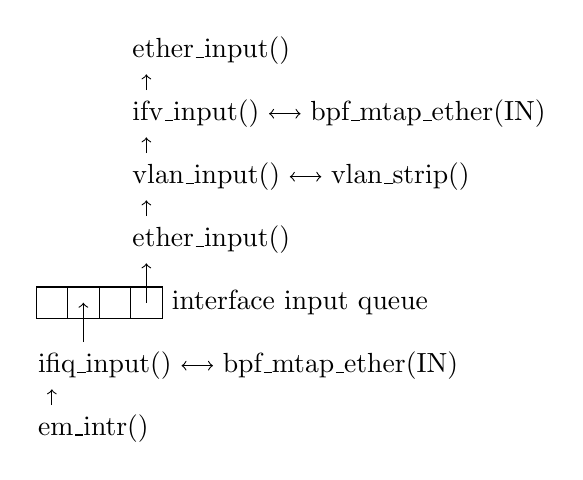
\begin{tikzpicture}
  \draw (0,0)
    node (em) [right] {em\_intr()} ++(0,.8)
    node (fq) [right] {ifiq\_input()} ++(.1,.6)
    rectangle ++(.4,.4) rectangle ++(.4,-.4)
    rectangle ++(.4,.4) rectangle ++(.4,-.4) ++(0,.2)
    node (iq) [right] {interface input queue} ++(-.5,.8)
    node (ev) [right] {ether\_input()} ++(0,.8)
    node (vi) [right] {vlan\_input()} ++(0,.8)
    node (fv) [right] {ifv\_input()} ++(0,.8)
    node (ei) [right] {ether\_input()}
    ;
  \path (node cs:name=em,anchor=west) +(.3,.3) coordinate (emo) {};
  \path (node cs:name=fq,anchor=west) +(.3,-.3) coordinate (fqi) {};
  \draw[->] (emo) -- (fqi);
  \path (node cs:name=fq,anchor=west) +(.3+1*.4,.3) coordinate (fqo) {};
  \path (node cs:name=iq,anchor=west) +(-.2-2*.4,0) coordinate (iqi) {};
  \draw[->] (fqo) -- (iqi);
  \path (node cs:name=iq,anchor=west) +(-.2,0) coordinate (iqo) {};
  \path (node cs:name=ev,anchor=west) +(.3,-.3) coordinate (evi) {};
  \draw[->] (iqo) -- (evi);
  \path (node cs:name=ev,anchor=west) +(.3,.3) coordinate (evo) {};
  \path (node cs:name=vi,anchor=west) +(.3,-.3) coordinate (vii) {};
  \draw[->] (evo) -- (vii);
  \path (node cs:name=vi,anchor=west) +(.3,.3) coordinate (vio) {};
  \path (node cs:name=fv,anchor=west) +(.3,-.3) coordinate (fvi) {};
  \draw[->] (vio) -- (fvi);
  \path (node cs:name=fv,anchor=west) +(.3,.3) coordinate (fvo) {};
  \path (node cs:name=ei,anchor=west) +(.3,-.3) coordinate (eii) {};
  \draw[->] (fvo) -- (eii);

  \draw[<->] (node cs:name=fq,anchor=east) -- +(.4,0)
    node (bm) [right] {bpf\_mtap\_ether(IN)};
  \draw[<->] (node cs:name=vi,anchor=east) -- +(.4,0)
    node (vs) [right] {vlan\_strip()};
  \draw[<->] (node cs:name=fv,anchor=east) -- +(.4,0)
    node (bv) [right] {bpf\_mtap\_ether(IN)};
\end{tikzpicture}
\end{frame}

\subsection{Hardware Transmit and Tcpdump}
\begin{frame}{Hardware Transmit and Tcpdump}
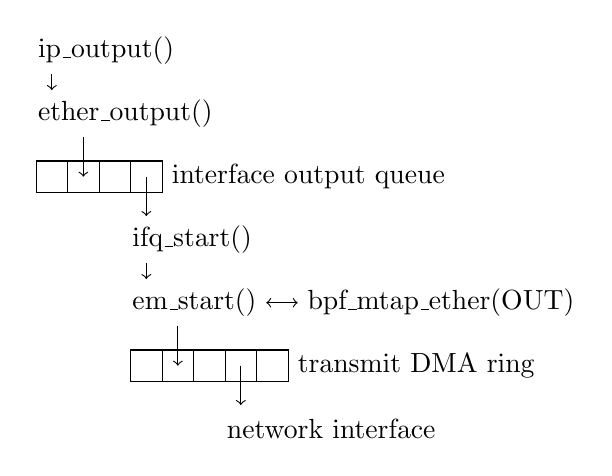
\begin{tikzpicture}
  \draw (0,0)
    node (io) [right] {ip\_output()} ++(0,-.8)
    node (eo) [right] {ether\_output()}  ++(.1,-.6)
    rectangle ++(.4,-.4) rectangle ++(.4,.4)
    rectangle ++(.4,-.4) rectangle ++(.4,.4) ++(0,-.2)
    node (oq) [right] {interface output queue} ++(-.5,-.8)
    node (fq) [right] {ifq\_start()} ++(0,-.8)
    node (es) [right] {em\_start()} ++(.1,-.6)
    rectangle ++(.4,-.4) rectangle ++(.4,.4)
    rectangle ++(.4,-.4) rectangle ++(.4,.4)
    rectangle ++(.4,-.4) ++(0,.2)
    node (tx) [right] {transmit DMA ring} ++(-.5-1*.4,-.8)
    node (ni) [right] {network interface}
    ;
  \path (node cs:name=io,anchor=west) +(.3,-.3) coordinate (ioo) {};
  \path (node cs:name=eo,anchor=west) +(.3,.3) coordinate (eoi) {};
  \draw[->] (ioo) -- (eoi);
  \path (node cs:name=eo,anchor=west) +(.3+1*.4,-.3) coordinate (eoo) {};
  \path (node cs:name=oq,anchor=west) +(-.2-2*.4,0) coordinate (oqi) {};
  \draw[->] (eoo) -- (oqi);
  \path (node cs:name=oq,anchor=west) +(-.2,0) coordinate (oqo) {};
  \path (node cs:name=fq,anchor=west) +(.3,.3) coordinate (fqi) {};
  \draw[->] (oqo) -- (fqi);
  \path (node cs:name=fq,anchor=west) +(.3,-.3) coordinate (fqo) {};
  \path (node cs:name=es,anchor=west) +(.3,.3) coordinate (esi) {};
  \draw[->] (fqo) -- (esi);
  \path (node cs:name=es,anchor=west) +(.3+1*.4,-.3) coordinate (eso) {};
  \path (node cs:name=tx,anchor=west) +(-.2-3*.4,0) coordinate (txi) {};
  \draw[->] (eso) -- (txi);
  \path (node cs:name=tx,anchor=west) +(-.2-1*.4,0) coordinate (txo) {};
  \path (node cs:name=ni,anchor=west) +(.3,.3) coordinate (nii) {};
  \draw[->] (txo) -- (nii);

  \draw[<->] (node cs:name=es,anchor=east) -- +(.4,0)
    node (bm) [right] {bpf\_mtap\_ether(OUT)};
\end{tikzpicture}
\end{frame}

\subsection{VLan Transmit and Tcpdump}
\begin{frame}{VLan Transmit and Tcpdump}
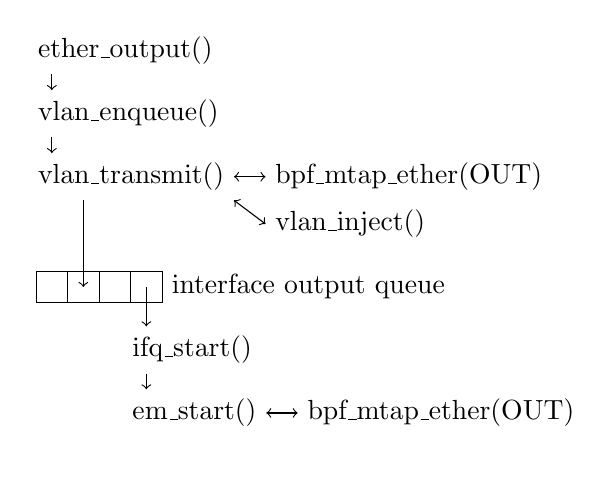
\begin{tikzpicture}
  \draw (0,0)
    node (eo) [right] {ether\_output()} ++(0,-.8)
    node (ve) [right] {vlan\_enqueue()} ++(0,-.8)
    node (vt) [right] {vlan\_transmit()} ++(.1,-.6-.6)
    rectangle ++(.4,-.4) rectangle ++(.4,.4)
    rectangle ++(.4,-.4) rectangle ++(.4,.4) ++(0,-.2)
    node (oq) [right] {interface output queue} ++(-.5,-.8)
    node (fq) [right] {ifq\_start()} ++(0,-.8)
    node (es) [right] {em\_start()} ++(.1,-.6)
    ;
  \path (node cs:name=eo,anchor=west) +(.3,-.3) coordinate (eoo) {};
  \path (node cs:name=ve,anchor=west) +(.3,.3) coordinate (vei) {};
  \draw[->] (eoo) -- (vei);
  \path (node cs:name=ve,anchor=west) +(.3,-.3) coordinate (veo) {};
  \path (node cs:name=vt,anchor=west) +(.3,.3) coordinate (vti) {};
  \draw[->] (veo) -- (vti);
  \path (node cs:name=vt,anchor=west) +(.3+1*.4,-.3) coordinate (vto) {};
  \path (node cs:name=oq,anchor=west) +(-.2-2*.4,0) coordinate (oqi) {};
  \draw[->] (vto) -- (oqi);
  \path (node cs:name=oq,anchor=west) +(-.2,0) coordinate (oqo) {};
  \path (node cs:name=fq,anchor=west) +(.3,.3) coordinate (fqi) {};
  \draw[->] (oqo) -- (fqi);
  \path (node cs:name=fq,anchor=west) +(.3,-.3) coordinate (fqo) {};
  \path (node cs:name=es,anchor=west) +(.3,.3) coordinate (esi) {};
  \draw[->] (fqo) -- (esi);

  \draw[<->] (node cs:name=vt,anchor=east) -- +(.4,0)
    node (bv) [right] {bpf\_mtap\_ether(OUT)};
  \draw[<->] (node cs:name=vt,anchor=south east) -- +(.4,-.3)
    node (vi) [right] {vlan\_inject()};
  \draw[<->] (node cs:name=es,anchor=east) -- +(.4,0)
    node (bm) [right] {bpf\_mtap\_ether(OUT)};
\end{tikzpicture}
\end{frame}

\section{IPsec}
\begin{frame}{Agenda}
\tableofcontents[currentsection]
\end{frame}

\subsection{IPsec Flow and SA}
\begin{frame}[fragile]{IPsec Flow and SA}
ipsecctl -s flow
\scriptsize
\begin{verbatim}
flow esp in
    from 10.188.108.0/24 to 10.188.115.0/24
    local fdd7:e83e:66bc:100::70 peer fdd7:e83e:66bc:100::17
flow esp out
    from 10.188.115.0/24 to 10.188.108.0/24
    local fdd7:e83e:66bc:100::70 peer fdd7:e83e:66bc:100::17
\end{verbatim}
\normalsize
ipsecctl -s sa
\scriptsize
\begin{verbatim}
esp tunnel
    from fdd7:e83e:66bc:100::17 to fdd7:e83e:66bc:100::70
    spi 0x10000861
esp tunnel
    from fdd7:e83e:66bc:100::70 to fdd7:e83e:66bc:100::17
    spi 0x10000862
\end{verbatim}
\end{frame}

\subsection{IPsec Input}
\begin{frame}{IPsec Input}
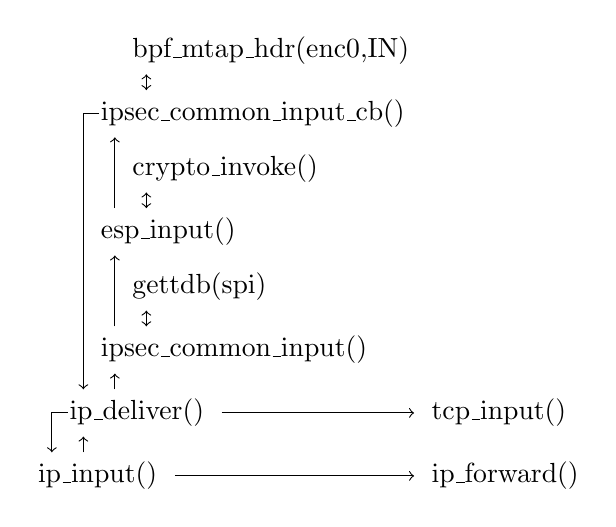
\begin{tikzpicture}
  \draw (0,0)
    node (ii) [right] {ip\_input()} ++(.4,.8)
    node (id) [right] {ip\_deliver()} ++(.4,.8)
    node (ci) [right] {ipsec\_common\_input()} ++(.4,.8)
    node (gt) [right] {gettdb(spi)} ++(-.4,.7)
    node (es) [right] {esp\_input()} ++(.4,.8)
    node (cr) [right] {crypto\_invoke()} ++(-.4,.7)
    node (cc) [right] {ipsec\_common\_input\_cb()} ++(.4,.8)
    node (be) [right] {bpf\_mtap\_hdr(enc0,IN)}
    ;
  \draw (5,0)
    node (if) [right] {ip\_forward()} ++(0,.8)
    node (ti) [right] {tcp\_input()}
    ;
  \path (node cs:name=ii,anchor=west) +(.7,.3) coordinate (iio) {};
  \path (node cs:name=id,anchor=west) +(.3,-.3) coordinate (idi) {};
  \draw[->] (iio) -- (idi);
  \path (node cs:name=id,anchor=west) +(.7,.3) coordinate (ido) {};
  \path (node cs:name=ci,anchor=west) +(.3,-.3) coordinate (cii) {};
  \draw[->] (ido) -- (cii);
  \path (node cs:name=ci,anchor=west) +(.3,.3) coordinate (cio) {};
  \path (node cs:name=es,anchor=west) +(.3,-.3) coordinate (esi) {};
  \draw[->] (cio) -- (esi);
  \path (node cs:name=es,anchor=west) +(.3,.3) coordinate (eso) {};
  \path (node cs:name=cc,anchor=west) +(.3,-.3) coordinate (cci) {};
  \draw[->] (eso) -- (cci);

  \path (node cs:name=cc,anchor=west) +(.1,0) coordinate (ccbo) {};
  \path (node cs:name=id,anchor=west) +(.3,.3) coordinate (idbi) {};
  \draw[->] (ccbo) -| (idbi);
  \path (node cs:name=id,anchor=west) +(.1,0) coordinate (idbo) {};
  \path (node cs:name=ii,anchor=west) +(.3,.3) coordinate (iibi) {};
  \draw[->] (idbo) -| (iibi);

  \path (node cs:name=ci,anchor=west) +(.7,.3) coordinate (cia) {};
  \path (node cs:name=gt,anchor=west) +(.3,-.3) coordinate (gti) {};
  \draw[<->] (cia) -- (gti);
  \path (node cs:name=es,anchor=west) +(.7,.3) coordinate (esa) {};
  \path (node cs:name=cr,anchor=west) +(.3,-.3) coordinate (cri) {};
  \draw[<->] (esa) -- (cri);
  \path (node cs:name=cc,anchor=west) +(.7,.3) coordinate (cca) {};
  \path (node cs:name=be,anchor=west) +(.3,-.3) coordinate (bei) {};
  \draw[<->] (cca) -- (bei);

  \path (node cs:name=ii,anchor=east) +(.1,0) coordinate (iifo) {};
  \path (node cs:name=if,anchor=west) +(-.1,0) coordinate (ifi) {};
  \draw[->] (iifo) -- (ifi);
  \path (node cs:name=id,anchor=east) +(.1,0) coordinate (idto) {};
  \path (node cs:name=ti,anchor=west) +(-.1,0) coordinate (tii) {};
  \draw[->] (idto) -- (tii);
\end{tikzpicture}
\end{frame}

\subsection{IPsec Output}
\begin{frame}{IPsec Output}
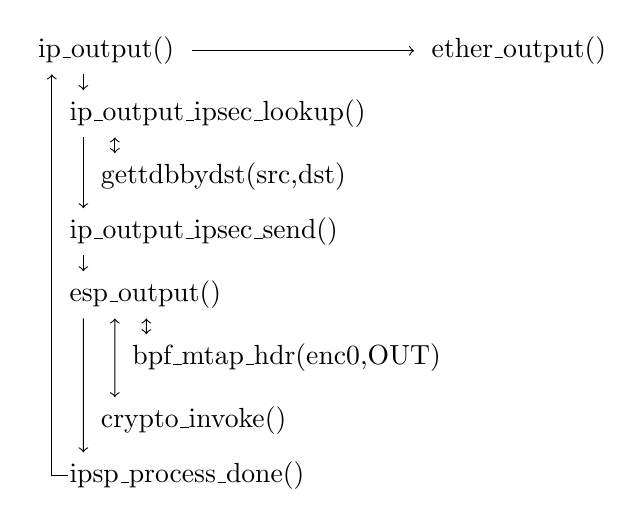
\begin{tikzpicture}
  \draw (0,0)
    node (io) [right] {ip\_output()} ++(.4,-.8)
    node (il) [right] {ip\_output\_ipsec\_lookup()} ++(.4,-.8)
    node (gt) [right] {gettdbbydst(src,dst)} ++(-.4,-.7)
    node (is) [right] {ip\_output\_ipsec\_send()} ++(0,-.8)
    node (es) [right] {esp\_output()} ++(.8,-.8)
    node (be) [right] {bpf\_mtap\_hdr(enc0,OUT)} ++(-.4,-.8)
    node (cr) [right] {crypto\_invoke()} ++(-.4,-.7)
    node (pd) [right] {ipsp\_process\_done()}
    ;
  \draw (5,0)
    node (eo) [right] {ether\_output()}
    ;
  \path (node cs:name=io,anchor=west) +(.7,-.3) coordinate (ioo) {};
  \path (node cs:name=il,anchor=west) +(.3,.3) coordinate (ili) {};
  \draw[->] (ioo) -- (ili);
  \path (node cs:name=il,anchor=west) +(.3,-.3) coordinate (ilo) {};
  \path (node cs:name=is,anchor=west) +(.3,.3) coordinate (isi) {};
  \draw[->] (ilo) -- (isi);
  \path (node cs:name=is,anchor=west) +(.3,-.3) coordinate (iso) {};
  \path (node cs:name=es,anchor=west) +(.3,.3) coordinate (esi) {};
  \draw[->] (iso) -- (esi);
  \path (node cs:name=es,anchor=west) +(.3,-.3) coordinate (eso) {};
  \path (node cs:name=pd,anchor=west) +(.3,.3) coordinate (pdi) {};
  \draw[->] (eso) -- (pdi);

  \path (node cs:name=pd,anchor=west) +(.1,0) coordinate (pdbo) {};
  \path (node cs:name=io,anchor=west) +(.3,-.3) coordinate (iobi) {};
  \draw[->] (pdbo) -| (iobi);

  \path (node cs:name=il,anchor=west) +(.7,-.3) coordinate (ilg) {};
  \path (node cs:name=gt,anchor=west) +(.3,.3) coordinate (gti) {};
  \draw[<->] (ilg) -- (gti);
  \path (node cs:name=es,anchor=west) +(1.1,-.3) coordinate (esb) {};
  \path (node cs:name=be,anchor=west) +(.3,.3) coordinate (bei) {};
  \draw[<->] (esb) -- (bei);
  \path (node cs:name=es,anchor=west) +(.7,-.3) coordinate (esc) {};
  \path (node cs:name=cr,anchor=west) +(.3,.3) coordinate (cri) {};
  \draw[<->] (esc) -- (cri);

  \path (node cs:name=io,anchor=east) +(.1,0) coordinate (ioeo) {};
  \path (node cs:name=eo,anchor=west) +(-.1,0) coordinate (eoi) {};
  \draw[->] (ioeo) -- (eoi);
\end{tikzpicture}
\end{frame}

\section{Tips \& Tricks}
\begin{frame}{Agenda}
\tableofcontents[currentsection]
\end{frame}

\subsection{Netstat Diff}
\begin{frame}[fragile]{Netstat Diff}
\begin{itemize}
  \item netstat -ss >before
  \item do some networking
  \item netstat -ss >after
  \item diff -up before after
\end{itemize}
\scriptsize
\begin{verbatim}
 tcp:
-       1024475 packets sent
-               829253 data packets (10075190801 bytes)
+       1024496 packets sent
+               829269 data packets (10075194870 bytes)
                8767 data packets (35352640 bytes) retransmitted
-               162711 ack-only packets (163607 delayed)
+               162715 ack-only packets (163619 delayed)
                21271 window update packets
\end{verbatim}
\end{frame}

\subsection{Grep Inet Counter}
\begin{frame}[fragile]{Grep Inet Counter}
\scriptsize
netstat -ss
\begin{verbatim}
ip:
        81 packets not forwardable
\end{verbatim}
grep 'not forwardable' /usr/src/usr.bin/netstat/inet.c
\begin{verbatim}
        p(ips\_cantforward, "\t%lu packet%s not forwardable\n");
\end{verbatim}
grep -l 'ips\_cantforward' /usr/src/sys/*/*
\begin{verbatim}
        /usr/src/sys/net/pf.c
        /usr/src/sys/netinet/ip_input.c
        /usr/src/sys/netinet/ip_var.h
\end{verbatim}
view /usr/src/sys/netinet/ip\_input.c
\begin{verbatim}
        if (!ISSET(flags, IP_FORWARDING)) {
                ipstat_inc(ips_cantforward);
                goto bad;
        }
\end{verbatim}
\end{frame}

\subsection{Counters}
\begin{frame}{Counters}
Developers should
\begin{itemize}
  \item check for error
  \item count errors
  \item use unique counter
\end{itemize}
\end{frame}

\section{Final Words}
\begin{frame}{Agenda}
\tableofcontents[currentsection]
\end{frame}

\subsection{Open Topics}
\begin{frame}{Open Topics}
\begin{itemize}
  \item routing
  \item arp, neighbor discovery
  \item bridge, veb
  \item hardware offloading
\end{itemize}
\end{frame}

\subsection{Links}
\begin{frame}{Links}
\begin{itemize}
  \item these slides
    {\small \url{https://github.com/bluhm/talk-packetflow}}
\end{itemize}
\end{frame}

\subsection{Questions}
\begin{frame}{Questions}
\begin{center}
\begin{tikzpicture}
\draw [font=\Huge] node {?};
\end{tikzpicture}
\end{center}
\end{frame}

\end{document}
